\documentclass[10pt,a4paper]{article}
\usepackage[utf8]{inputenc}
\usepackage{tabularx}
\usepackage{enumitem}
\usepackage{microtype}
\usepackage{url}
\usepackage[backend=bibtex8,sorting=none]{biblatex}
\usepackage{pdfpages}
\usepackage{listings}
\usepackage{color}
\usepackage{tikz}
\usepackage{hyperref}

% set up syntax highlighting for listings
\definecolor{lightgray}{rgb}{.95,.95,.95}
\definecolor{darkgray}{rgb}{.4,.4,.4}
\definecolor{purple}{rgb}{0.65, 0.12, 0.82}
\lstdefinelanguage{JavaScript}{
  keywords={typeof, new, true, false, catch, function, return, null, catch, switch, var, if, in, while, do, else, case, break},
  keywordstyle=\color{blue}\bfseries,
  ndkeywords={class, export, boolean, throw, implements, import, this},
  ndkeywordstyle=\color{darkgray}\bfseries,
  identifierstyle=\color{black},
  sensitive=false,
  comment=[l]{//},
  morecomment=[s]{/*}{*/},
  commentstyle=\color{purple}\ttfamily,
  stringstyle=\color{red}\ttfamily,
  morestring=[b]',
  morestring=[b]"
}
\lstset{
   language=JavaScript,
   backgroundcolor=\color{lightgray},
   extendedchars=true,
   basicstyle=\footnotesize\ttfamily,
   showstringspaces=false,
   showspaces=false,
   numbers=left,
   numberstyle=\footnotesize,
   numbersep=9pt,
   tabsize=2,
   breaklines=true,
   showtabs=false,
   captionpos=b
}

% add the file containing our references
\addbibresource{main.bib}

% include shapes and arrows for flow charts and set up
\usetikzlibrary{shapes.geometric, arrows}
\tikzstyle{startstop} = [rectangle, rounded corners, minimum width=3cm, minimum height=1cm,text centered, draw=black, fill=red!30]
\tikzstyle{io} = [trapezium, trapezium left angle=70, trapezium right angle=110, minimum width=3cm, minimum height=1cm, text centered, draw=black, fill=blue!30]
\tikzstyle{process} = [rectangle, minimum width=3cm, minimum height=1cm, text centered, draw=black, fill=orange!30]
\tikzstyle{decision} = [diamond, minimum width=3cm, minimum height=1cm, text centered, draw=black, fill=green!30]
\tikzstyle{arrow} = [thick,->,>=stealth]

% document info
\title{Building a Decentralised Taxi App}
\author{Scott Street\\{\small 159027651}}
\date{April 2018}

\begin{document}

\maketitle

% TODO: write the abstract
\abstract{Decentralised apps are pretty cool, but they don't quite work the same as what we're used to.}

\tableofcontents

\pagebreak

\section{Introduction}

Taxicoin is an attempt at designing and building a protocol for hailing taxis, where the entire system is fully decentralised, with no single authority in control. The motivation behind this is to combat some of the issues found with existing similar traditional applications, such as \textit{Uber} and \textit{Lyft}.

These companies saw a way to improve the taxi industry, and by improving the user experience and ease of ordering a taxi, attracted many users. However, as was the case with existing taxi companies, they still take a significant cut of fares. Coupled with the fact that they attempt to keep fares lower for passengers, the drivers are left with very little earnings.

In contrast, Taxicoin has been designed so that the will of riders and drivers self-regulates fares. A driver decides and quotes fares on an individual basis, rather than being instructed as to what fare they should charge. Riders then only accept fares that they feel are fair -- if they are in a hurry, they may be willing to pay a higher price.

\subsection{Benefits of Decentralisation}

In general, decentralised systems are more open. In context, this means that anybody is free to participate -- one of the key precepts of Taxicoin.

Additionally, such systems, if designed well, should be not in the control of any one group of people. If we look at traditional taxi companies, the customers are at the will of the company. In many cases, one company will form the sole taxi coverage of a territory, meaning that they can decide on the price for a journey.

With a decentralised system, decisions about such issues are made transparently between all parties involved. In short, decentralisation creates a fairer system.

\subsection{Why an Open Protocol}

Continuing with the themes of decentralisation, it was important that Taxicoin be as open as possible. If a single entity was tasked with developing and maintaining the Taxicoin network, and decided to cease doing so, the entire system would likely collapse. It also creates a \textit{walled garden} scenario, where the single entity has total control over the system. They could decide at any point to disregard the original decisions made behind the network, and start charging a fee for each journey.

But with an open protocol, the specification needed to implement ones own version of Taxicoin is freely available. If users in a certain location beyond that which is actively supported by the initial version wish to launch their own Taxicoin, they can. It also allows for continued critique and improvement, where potential bugs can be discovered and fixed, and if a developer external to the original project wishes to write an extension to the protocol to add further features, they may do so.

\section{An Explanation of Ethereum}

Ethereum is a platform consisting of three components: Swarm, a “distributed storage platform and content distribution service” \cite{Swarm}; Whisper, a peer-to-peer communication protocol \cite{Whisper}; and the Ethereum Virtual Machine (EVM) used for running smart contracts \cite{Ethereum}. The latter is often referred to alone simply as “Ethereum”, however all three should be considered part of the same platform, each one complimenting the others. The aim of this section is to explain how these three solutions are used together to develop fully decentralised applications, or dApps.

\subsection{Blockchains}

The EVM component of Ethereum is built on top of a “blockchain”, a term coined by the anonymous creator of Bitcoin \cite{Bitcoin}, which is the original, and most widely known application of such technology. At its core, a blockchain consists of transactions, grouped together into “blocks”, with each group also referencing the previous one, thus forming a “chain”. A blockchain can be thought of simply as a form of database, keeping a state. A transaction represents a state transition, but must be verified before being deemed to be valid and placed in a block.

% TODO: blockchain diagram here?

The blockchain itself is distributed across all nodes in the network (except in cases where a node chooses to reference another’s copy), meaning that, unless explicitly obfuscated by the user, all transaction data on the network is open. This allows the auditing of transactions by any node on the network, and eliminates the need to trust a single entity to provide accurate data - this is the concept of trustlessness.

Transactions on the Bitcoin blockchain are, for the most part, simply that - transactions. They represent a transfer of funds from one "address" to another. They can additionally contain an amount of data, representing anything from a simple message, to a method call in cases where the receiving address is a “smart contract" (or simply “contract”).

In Bitcoin, contracts are a special type of address which causes nodes on the network to execute some predefined code when a transaction is sent to it. Contracts are deployed by a standard (human controlled) address, but once deployed act as independent entities. Unless their code contains functionality to do so, the deployer has no control over the contract.

However, contract execution on the Bitcoin network is not Turing complete, due to the halting problem - the inability to determine whether a section of code will complete execution without looping infinitely. If contract execution was Turing complete in the existing Bitcoin network, a malicious actor would be able to perform a denial of service attack against the network by deploying and calling contact code containing an infinite loop.

This is where the EVM differs, with the addition of “gas”. This introduces a fee per instruction to be executed (paid in Ethereum’s native cryptocurrency, Ether). The sender of a transaction sets the maximum amount of gas they are willing to spend for a transaction to complete, and a contract call will continue executing until either the execution completes, or the maximum amount of gas is consumed. This safely allows the use of loops within contracts, as it becomes very expensive to perform an infinite-loop attack.

The result is that the EVM is Turing complete, and thus in theory any arbitrary program can be implemented in a contract, opening the door to a wide variety of applications.

\subsection{dApps}

While smart contracts are well suited to taking inputs, making state changes, and producing outputs, that is all they do. It is possible to interact with them via a command line interface, through an Ethereum node, however this is obviously far from the desired experience for end users. To address this problem, several attempts at providing a user interface layer for the Ethereum network have been introduced. The most widely adopted, and officially endorsed solution, is Web3 - a browser API which allows interacting with all parts of the Ethereum platform from Javascript embedded on a web page.

This leads to the approach that many Ethereum dApp developers take: considering their application as a traditional “Single Page App”, where instead of calling HTTP API endpoints, they are now interacting with a smart contract through the use of Web3. Smart contracts effectively take the place of a “backend” web server, leading to many benefits over traditional web apps, such as availability, security and integrity.

Coupling this with Whisper allows for peer-to-peer communication between instances of a dApp, which in most cases translates to between different users. For example, two parties negotiating the price of an item to be purchased - they do not necessarily want their negotiation to be public (or rather, it does not provide any value for it to be), therefore they can come to an agreement “off-chain” before publishing (sending) a transaction of the final agreed price. Whisper is also beneficial for situations where the sender of a message wishes to remain anonymous. When publishing a transaction on the blockchain, the sender is published along with it, whereas in Whisper, unless signed, it is improbable to determine the sender of a message [cite]. % TODO: cite shh plausible deniability

Additionally, the static HTML, Javascript and any additional components of a dApp can be hosted from Swarm (or a similar platform such as IPFS [cite]). When a file, or set of files, is published to Swarm, a hash is computed, and the file is split into pieces called “shards”. The shards are then distributed across nodes in the network, with the intention that if one node becomes unavailable, the shards of the file should still be accessible. When a user wishes to retrieve a file at a later date, they can provide the previously computed hash to a Swarm node, which will request shards of the file from its connected peers. % TODO: cite IPFS

In this manner, it is possible with the Ethereum platform to develop fully decentralised applications where the user interface is written as a web page and is served from Swarm, thus eliminating the requirement for a traditional web server. An application’s “backend” logic is contained within a smart contract, removing the need for a backend web server such as PHP. And finally, instances of the application may communicate between each other through the use of Whisper, removing the need for a solution such as WebSockets, where a central signalling server is required.

\subsection{Smart Contract System Design}

As smart contract execution is only ever triggered as a result of a transaction, applications must be designed around deliberate actions. For example, where in a traditional system, a method may be set to execute at a particular date and time, in a smart contract this is not possible. Instead such a method may only have a check for if the allowed time of execution has passed, and must be manually triggered by a transaction.

As the reasons for some of these differences are unlikely to be clear to users, it is important to consider how to communicate them.

Additionally, as there is an attached "gas" fee for publishing transactions and calling contract methods, it is in the interests of the users for the contract developer to make contracts as efficient as possible, and to make a minimal number of contract calls in a dApp. One way of doing this is to avoid on-chain interaction wherever possible, through the use of peer-to-peer protocols, predominantly Whisper. In extreme cases, complex routines within contracts can be written in the underlying EVM byte-code for improved efficiency.

\section{Identification of Requirements}

The first step towards developing Taxicoin was to identify the requirements for the resulting system. These were split into two categories: minimum viable and additional requirements.

\subsection{Minimum Viable Requirements}

These requirements are those which must be included in order for the system to correctly function.

\bigskip\textbf{Drivers must be required to pay a deposit in order to advertise} to act as a reasonable barrier to entry. Without this in place, the network is easily open to spam and scammers posing as drivers. The deposit acts as an incentive to behave well.

\bigskip\textbf{Riders must advertise jobs to drivers on an individual basis} in order to protect the privacy of the rider. As this is likely to contain individually identifying information, such as location, if this were published it could be used to track an individual.

\bigskip\textbf{The fare must be determined by quotes from driver} to remove the need for a centralised fare decision. This is due to the fact that the fare depends on many factors which cannot be automatically determined in a decentralised and reliable manner, such as distance and demand. The alternative would be fixed fares, but this is highly undesirable as short trips would be overpriced, and long trips underpriced.

\bigskip\textbf{Riders must pay fares to a contract in advance} as a security measure, due to the fact that there is no other way to guarantee riders will pay after the fact. Without this, it is likely that a subset of riders would not pay for journeys.

\bigskip\textbf{Riders must provide an additional deposit before starting a journey} to act as an incentive to successfully and formally complete a journey in the system. Without this, riders may have paid fare and have no regard for consequences of bad acts. Additionally, they may not carry on to rate the driver, an integral part of the smooth running of the system.

\bigskip\textbf{Riders and drivers must both rate the other on completion of a journey} to affect the reputation of the other party. This is likely to be implemented such that a user is unable to interact with the rest of the system until they have formally completed their previous journey. Without this requirement, there is no way to determine the trustworthiness of another individual on the network, which is key to preventing bad behaviour.

\bigskip\textbf{When a journey is completed, deposits should be returned to the respective parties, and the fare paid to the driver} this ensures that riders and drivers both have a stake in formally completing a journey. If they do not, their deposits are not returned, and neither is the driver paid. Without this deposit system, there is no guarantee that either party will rate the other - potential hit-and-run scenarios could occur where a rider uses the system only once and does not care to formally complete a journey and rate their driver as it provides no benefit to them. With the deposits however, they are likely to complete the process, at stake of losing their funds.

\subsection{Additional Requirements}

These are requirements deemed as \enquote{nice to have} features, without which the system will continue to function, but the addition of which would improve the system in some way.

\bigskip\textbf{Prospective drivers and riders should be able to informally communicate before forming a contract} to allow any additional requirements on either part be known. For example if a rider is wishing to take a large, bulky item on the journey with them, they may communicate this in advance. If it transpires that the driver's car is small, the journey can be cancelled (or not formally begun), and another driver arranged, before the original driver has taken the effort of travelling to pick up the rider.

\bigskip\textbf{Dispute resolution should be built into the system} for situations where driver and rider are unable to successfully complete a journey. This would work in a similar way to negotiating a price. In a worst case scenario, the driver wants payment in full, but the rider wants to pay nothing. In this case, the two negotiate until an agreement is reached. If they do not reach such an agreement, it reflects poorly on both parties, as the fact that they have an unresolved dispute is public. The system is able to function without this, but bad disputes are likely to go unresolved which is dissatisfactory.

\section{Protocol Specification}

The protocol portion of Taxicoin is designed to be open. As such, anybody should be able to implement it in their own software. The following section of this document should be sufficient to do so.

\subsection{Methods}

Each of these methods is intended to be part of a smart contract. When one is called, it will modify the state of the contract, and/or return a value.

The specified arguments are to be supplied when calling that function of the contract. The \textit{payable} keyword indicates that a method accepts a transaction with a currency value attached.

\subsubsection{Driver Advertise}

\begin{description}
	\item [Arguments] latitude; longitude; Whisper identity
	\item [Payable] driver deposit value, defined in contract
\end{description}

The advertise method takes a location and deposit (value as defined by the contract settings) from a driver and the contract publishes the location of the driver.

If a deposit has not already been provided, and is not sent with the advertisement, an error is thrown. If deposit is sent, but has already been provided, the excess is returned and the method returns successfully.

\subsubsection{Driver Advert Revoke}

\begin{description}
	\item [Arguments] none
	\item [Payable] no
\end{description}

If an active advertisement exists, its state is set to invalid, indicating that riders should not consider this driver. Deposits are not returned as a result of this action.

\subsubsection{Rider Create Journey}

\begin{description}
	\item [Arguments] driver address, fare
	\item [Payable] fare plus rider deposit value, defined in contract
\end{description}

Accepts a quoted fare for a journey as a rider and forms contract between driver and rider, taking full fare plus deposit from rider.

The contract is not complete until the driver formally accepts the job by calling the accept journey method. Before this happens, the journey may be cancelled with no adverse effect for the rider, with the fare and deposit being returned in full.

This is intended to be called after an off-chain negotiation, with job proposal and quote messages.

\subsubsection{Driver Accept Journey}

\begin{description}
	\item [Arguments] rider address
	\item [Payable] no
\end{description}

Formally accepts a job, committing both the rider and driver to its completion (or otherwise amicable resolution) at the stake of the fare and deposits.

If the rider, as identified by the given address, has not initiated a journey contract, then the method will return an error.

\subsubsection{Complete Journey}

\begin{description}
	\item [Arguments] none
	\item [Payable] no
\end{description}

Marks the current journey as completed, as either the rider or driver. The journey will not be fully complete until both parties have called this method.

Once the journey is complete, the fare is paid from the contract to the driver, and deposits are returned to both parties.

\subsubsection{Cancel Journey}

\begin{description}
	\item [Arguments] none
	\item [Payable] no
\end{description}

Proposes the cancellation of a journey, or in the case that the other party has already proposed a cancellation, accepts the proposal.

The fare is returned from the contract to the rider, along with the rider's deposit. The driver's deposit is not returned.

\subsection{Messages}

Driver and rider user clients should be listening for the following messages, where applicable. These messages are communicated via the Whisper protocol.

Message topics are always a length of 4 bytes (4 ASCII characters), therefore any topics listed here of a length less than 4 byes are right-padded with spaces.

\subsubsection{Job Proposal}

\begin{description}
	\item [Topic] job
\end{description}

This message is sent by a rider to a prospective driver, indicating that they wish to make the described journey. It is intended to be sent to advertised drivers matching a specified criteria, e.g. within a certain distance, with at least a certain reputation. However the sending of these messages is not intended to be carried out manually by the user -- rather there is an automated process which fetches the list of active drivers and determines which to propose to.

The payload consists of an ASCII string of a stringified JSON object containing \lstinline{pickup} and \lstinline{dropoff} locations, as well as the network (Ethereum) address of the rider.

\lstinputlisting{res/job-message.json}

Should a driver be interested in a proposal, they respond with a quote message.

\subsubsection{Driver Quote}

\begin{description}
	\item [Topic] quot
\end{description}

This message is sent by a driver as a response to a job proposal. It contains the network address of the driver, as well as the fare for which the driver is willing to take on the job. At this point, the quote is not binding.

\lstinputlisting{res/quote-message.json}

If the rider chooses to accept the quote, they next call the create journey method.

\subsection{Process Flow Diagram}

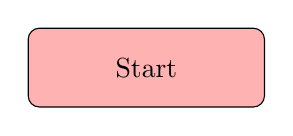
\begin{tikzpicture}[node distance=2cm]
	\node (start) [startstop] {Start};
\end{tikzpicture}

\section{Implementation}

My implementation is in two parts: that of the protocol described above, and additionally an example \textit{Web3} client. The protocol itself is split between peer-to-peer communication and smart contract methods. P2P messages are handled entirely outside of the contract, and in this implementation are sent by the client library via the Whisper protocol on the Ethereum network.

The entire implementation of the Taxicoin protocol and client is contained within one git repository. The directory structure is defined by a combination of \lstinline{vue-webpack} \cite{VueWebpack} and \lstinline{truffle} \cite{Truffle}, both of which have strong opinions.

\subsection{Smart Contract}

As previously discussed, Ethereum smart contracts are self-contained programs which execute on the Ethereum Virtual Machine (EVM). The core of Taxicoin is implemented as a contract, allowing riders and drivers to interact with one and other with it as an intermediary.

The contract is centred around state, which can be divided into three parts: the state of the Taxicoin network, the state of a driver, and the state of a rider. It conforms to the \lstinline{TaxicoinInterface} contract interface, as defined in the protocol specification.

\subsubsection{Network State}

When a contract is deployed, various parts of it may be initialised, in a similar way to how the constructor of a class initialises the state of an object. In Taxicoin, only the driver and rider deposit values are set at this stage.

Two key mappings are kept: one which maps an address to a driver, and one which maps an address to a rider. There is additionally a third mapping used to implement a double-linked list (DLL), discussed below.

There is also a \lstinline{UserType} enum from the contract interface, which is used as a return type for the \lstinline{getUserType} helper function. This is an easy method of determining the current \enquote{mode} of a user based on the state of their \lstinline{Driver} and \lstinline{Rider} objects (described in more detail below).

\lstinputlisting[language=Solidity]{res/user-type-enum.sol}

\subsubsection{Driver State}

An individual driver is represented by a \lstinline{Driver} struct:

\lstinputlisting[language=Solidity]{res/driver-struct.sol}

When a user first wishes to become a driver, a \lstinline{Driver} object will not exist for them\footnotemark, and they will have to call the \lstinline{driverAdvertise} method, providing their current latitude, longitude, Whisper public key (used for peer-to-peer communication), and a deposit. If the deposit provided is sufficient, then the driver's state will be updated.

\footnotetext{Rather, the mapping will return a Driver object with all zero values.}

This consists of setting the address of the driver on the object (used as an integrity check - the address of an advertised driver should map to a \lstinline{Driver} object with the same address), the latitude and longitude, the time at which the driver was last updated (used to detect stale advertisements), the deposit provided by the driver (for cases where the global driver deposit value may change, the amount provided when the driver initially advertised is what will be returned), and the driver's public key (used for contacting this driver via Whisper). Additionally, if the driver is not already advertised, their address is added to the DLL.

Just as the address of a \lstinline{Driver} object is used to check integrity, it is also used to indicate whether a driver is currently advertised or not. Any user should be able to view information about a driver at any time, and the overall rating of a driver needs to be stored even while a driver is not advertised. Therefore, this data is kept, and can be accessed via the \lstinline{drivers} map. However, if the address does not match, this indicates that the driver is not currently advertised.

To mark a driver as not active, they are removed from the DLL and their address set to zero. To mark a driver as on a journey, they are removed from the DLL and their rider is set to a non-zero address. The advantage of this state-based approach to determining the mode of a driver is that we do not have to explicitly store and update a separate indicator.

\subsubsection{Rider State}

An individual rider is represented by a \lstinline{Rider} struct:

\lstinputlisting[language=Solidity]{res/rider-struct.sol}

A rider's rating and rating count are kept between journeys, but otherwise, all remaining fields are empty when the rider is not part of a journey. As with a driver, the \lstinline{addr} field is used to determine whether a rider is active. To determine whether the driver is locked into a journey, we look up the driver in the \lstinline{drivers} mapping, using the given address. If their rider field is set to the address of this rider, then both users are locked into a rider together.

\subsubsection{Double Linked List}

As Solidity is still a relatively young language, some features which one would expect from a more mature language are missing. This includes the ability to return dynamic-length lists from a method, which posed an issue early in the development of Taxicoin. Although it's possible to return a single element at a time, this requires keeping a separate cursor for which element should be next. Therefore we instead use a novel implementation of a double-linked-list, which allows us to use the address of the current driver as the cursor to fetch the next or previous\footnotemark.

\footnotetext{The ultimate implementation was based on \cite{DLL}.}

Modifying operations on the list are likely be performed on only a single element at a time, therefore to link to the next and previous item in the list is not much more of a cost. This provides the benefit of not having to scan forward to move backwards in the list, particularly useful for pagination, which will likely be needed when a large number of drivers are advertised and a user wishes to manually review potential drivers.

The contract uses a mapping which maps driver addresses to another map, which in turn maps a boolean to an address. The boolean represents whether we want to look up the next or previous element in the list - false is the previous, and true is the next. This then returns the address to use to look up the \lstinline{Driver} object in the drivers mapping.

This list is easily interfaced with using the \lstinline{getNextDriver} and \lstinline{getPreviousDriver} methods, as defined in the contract interface. These features of the protocol were in fact partly designed this way due to the limitation as described above, that solidity does not support returning dynamic-length lists from methods.

\subsubsection{Journeys}

Building on the idea of rider and driver state, there is no concrete \textit{journey} object in this Taxicoin implementation. Rather, the concept of a journey is inferred from the state of the participants.

When observing a rider, if the \lstinline{driver} property is set, this indicates that the driver is either on a journey with that driver, or has created the journey and is waiting for the driver to accept. Whether the driver has accepted or not can be determined by observing the driver's \lstinline{rider} property. If it is set the address of the rider, then the driver has accepted the journey and both are formally part of the same journey. If the driver's rider address is blank, they have not yet accepted the journey, and if it is the address of another rider, then they have effectively declined the journey with this rider and have chosen to accept another rider's journey.

At the end of a journey, both parties call the \lstinline{Complete Journey} method, which will record the rating to be given to the other. This is stored in the rider/driver object for the user, and additionally acts as an indication as to whether the user has already called the method. This is then used by the method to determine whether to finalise the completion of the journey.

When both parties have completed the journey, the ratings given are applied (recalculate average rating, and increment rating count), deposits returned, and the fare paid to the driver. The state of both is then reset -- their own addresses and those pointing to the other are set to zero, the ratings to be given to the other are set to zero, and the recorded values for the deposits are fare are set to zero.

\subsubsection{Integrity Checks}

As this implementation is heavily based on the state of objects within the contract, it is important to maintain data integrity. Coupled with the immutability of smart contracts, if we do not ensure that our contract state is kept correctly, it may be impossible to recover from a situation where the state is altered in some unexpected way.

A key feature of Solidity which allows us to check certain pre- and post-conditions is the use of \lstinline{require();}. In the case that the contained statement evaluates to false, execution will halt and any changes made to the state of the contract instance are reverted.

For example, the protocol specification states that when a driver advertises, they must first be required to pay a deposit. Additionally, they may not already be on a journey as either a driver or rider. To check these post-conditions we can use the following Solidity code:

\begin{lstlisting}[language=Solidity]
// check the driver has paid deposit
require(drivers[msg.sender].deposit >= driverDeposit || msg.value >= driverDeposit);

// must not be ActiveDriver or Rider
require(getUserType(msg.sender) != UserType.ActiveDriver);
require(getUserType(msg.sender) != UserType.Rider);
\end{lstlisting}

This is also useful for performing \enquote{safe math}, where we want to protect against overflow or underflow. In both of these cases, integers in Solidity will simply wrap-around, which, particularly when dealing with currency as is the case much of the time in Solidity, can be catastrophically bad. Although it may not always be possible to recover from a situation where over- or underflow would occur, we can use \lstinline{require} to check if the resulting value has been a result of such an occurrence, and revert the state of the contract instance.

\subsection{Client Library}

While the contract handles the state of Taxicoin, it can be unwieldy to interact with. It also only implements part of the Taxicoin protocol, not including any of the off-chain, peer-to-peer interactions.

The JavaScript client library is what really opens up the potential ecosystem of applications using the Taxicoin protocol. The aim was for it to be as simple to use and integrate into other people's projects as possible, and ideally should hide as much of the complexity of interacting with an Ethereum smart contract as possible.

The client library exposes a class, which when instantiated sets up all of the common requirements for using the Taxicoin protocol in most cases.

\subsubsection{Web3 Interaction}

The JavaScript library used for interacting with the Ethereum blockchain is called \lstinline{Web3.js} \cite{Web3}, and acts as a layer for sending commands to an Ethereum network node which computes transactions and relays them to the network.

This is coupled with the \lstinline{truffle-contract} library, which abstracts the logic for calling methods of a smart contract, and provides each one as an asynchronous JavaScript method. These in turn interact with a Web3 library instance. The typical code\footnotemark for calling a contract method is as follows:

\footnotetext{In ES6 async/await function syntax.}

\begin{lstlisting}
const instance = await this.contract.deployed()
const account = await this.getAccount()
const tx = await instance.methodToCall([arguments, ]{from: account[, otherOptions})
\end{lstlisting}

\lstinline{this.contract} is a \lstinline{TruffleContract} instance which points to the Taxicoin contract code. Calling the \lstinline{deployed} method on that returns a wrapper with a reference to a deployed instance of the contract on the current network. From this, we can then call the methods of the deployed contract.

The \lstinline{getAccount} method fetches the Ethereum address of the user, as defined when instantiating a Taxicoin library instance. This is then required to be passed as an option with any contract method calls which modify state, as it is used to identify the user when signing the transaction.

\subsubsection{Peer to Peer Messages}

The other key purpose of the client library is to facilitate the sending of peer-to-peer Taxicoin protocol messages. This is done with Whisper, one of the protocols part of the Ethereum network.

As Whisper is a fairly low-level protocol, sending messages is not entirely straightforward. The Web3 library handles much of the work, however it still requires various parameters, such as keys and the level of encryption it should use. Topics in Whisper also must be exactly 4 bytes in length, and the Web3 library expects this as a hexadecimal string, which is not something that would be straightforward for a user of the Taxicoin library.

Therefore, the library manages the keypair for use with Whisper, maps human-readable topic names to 4 byte hexadecimal string, converts JSON objects to strings for sending as the payload of a message, and handles the various other parameters used when sending Whisper messages.

For messages which are intended to be send after certain on-chain actions are taken, the library handles this, waiting for the transaction to be confirmed, and sending the appropriate message.

The library also registers filters for the various Taxicoin message topics, automatically polls for new messages sent to the user, and fires JavaScript events which the user of the library may listen for in their application.

\subsection{Example Web Client}

The example client implementation uses the client library, along with \textit{Web3.js} to interact with the Ethereum blockchain and Whisper protocol.

The \textit{Vue.js} JavaScript framework is used as a basis on which to develop a single-page web application. Vue uses a component-based architecture, where the functionality and formatting for a component is all self-contained. Pages are also considered to be components, and therefore each page follows the same model.

The application is split into two main parts: the ride page, and the drive page. Each one features user interface elements specific to that type of user.

\begin{figure}[h]
	\centering
	\includegraphics[width=11cm]{res/webapp.png}
	\caption{The example Taxicoin client, as viewed in the Safari browser.}
\end{figure}

Vue introduces the concept of \textit{reactive} data - when a JavaScript object changes value, any component which is using the data (observing it) automatically updates to use the new value. Retrieving the user's current location is a key requirement for any implementation of the Taxicoin protocol, and within a web browser this can be done using the geolocation browser API.

To adapt this for use with Vue's reactive models, a Vue \textit{plugin} has been created as part of this implementation. This creates a \lstinline{$location} object available to all components globally, which has latitude and longitude components, both of which are reactive.

Another plugin was also created for exposing a Taxicoin library instance to all components. This means that instead of needing to instantiate this for each page components and then pass it to child components where needed, the one instance is available globally.

Although this client implementation is functional, it is not feature complete at the time of writing, and does not implement all features of the library, such as sending of the driver's location to the rider, or a user interface for proposing a fare alteration. However, it is sufficient as a proof of concept.

Additionally, this application is most likely to be used from a mobile device (very few taxi drivers carry a laptop with them). This is possible using the Status mobile Ethereum browser \cite{Status.im}, which exposes a Web3.js object to web pages (also including Whisper protocol functionality, and in fact pioneering the 6th iteration of the protocol).

\section{Testing and Validation}

\subsection{Unit Tests}

\subsection{Static Analysis}


\pagebreak

\printbibliography[heading=bibintoc]
\pagebreak

\section*{Appendix}
\addcontentsline{toc}{section}{Appendix}

\subsection*{Project Definition}
\addcontentsline{toc}{subsection}{Project Definition}

\subsubsection*{Subject}

When the Internet was in its infancy, if you wanted to use it for a specific application, you might have written a protocol. That way, anybody who wanted use the Internet for that purpose would have a common way of doing it - and if a new person came along and wanted to join in, they could just write their software to conform with the standard.

In the past 15-or-so years however, the landscape has changed. Companies now favour their own proprietary systems, where they can have complete control, and ultimately gain the most profits. Specifically companies such as Uber have taken an industry which was once fairly well distributed, and put the control in their own hands - they decide who can be a driver, they manage the fares, and how much they pay their drivers.

But recent developments with distributed networks threaten to disrupt this comfy business model. Technologies such as Ethereum allow "trustless" applications, where activities of a single node are verified by the entire network. It's an area which is yet to be explored to its full potential, but all the features needed to be able to implement feature-rich apps are there. The logic of applications running on such a system has to be rethought, but with Uber as an example, there would be no central authority to take a cut of profits. The entire system would be self-regulating.

\subsubsection*{Deliverable}

A ride-sharing webapp accessible with an Ethereum network-enabled browser, designed in such a way that no single entity has control over the running of the system. Drivers will be able to advertise their location (published to blockchain), and riders will be able to send job proposals (containing pickup and drop-off locations) to these drivers on a peer-to-peer basis. This protects the privacy of the rider by ensuring that only the chosen drivers are able to see the rider’s location. When a driver initially advertises their location, they are required to provide a deposit to the network, which will be returned in completion of a trip. This gives the driver a stake in wanting to complete a journey, and should reduce spam on the network.

Drivers are then able to issue a response to a proposal, by either rejecting or quoting a price for the journey. This allows drivers to choose which journeys they take, and prevents drivers from having to travel a long distance to a pickup location, compared with if the allocation was done randomly. Should the rider choose to accept the quote, then both rider and driver form an agreement via a smart contract on the Ethereum network. This includes the passenger offering up the cost of the journey, plus an additional deposit equal to the amount the driver provided previously.

At this point, the fare for the journey, a deposit from the rider, and a deposit from the driver are all held by a smart contract. This acts as an incentive for the driver and rider to successfully complete the physical journey. When this is done, and both parties are in agreement that it is completed, then the deposits can be returned and the fare paid to the driver.

All monetary transactions will be executed with cryptocurrency on the Ethereum network, so as to minimise fees and prevent the transaction from being intercepted by a third party.

As the vast majority of interactions between riders and drivers will be based on no existing knowledge of the other party, a reputation system will be used to form a layer of trust. Based on previous journeys, and the ratings given to both rider and driver on completion of each, future riders will be able to make informed decisions about which drivers to send job proposals. And in the same fashion, drivers will be able to decide which riders’ proposals to accept.

\subsubsection*{Originality}

Although ride-sharing apps aren’t a new thing, nearly all existing solutions are controlled by a central authority who take a cut of the profits. This means users are at the mercy of the company when it comes to fares, and drivers must be approved, potentially opening the way for discrimination.

This project eliminates these problems by taking control away from any one part of the system. All transactions take place in a peer to peer nature, with the network being the only intermediary. This ensures that the two parties involved have full control over the process, whilst at the same time preventing one from cheating the other.

\subsubsection*{Timetable}

The following proposed timetable will be used to track progress over the course of the project. The work is broken down into fortnightly blocks. Through the entirety, a project diary will be kept to keep track of key decisions. This is to be used as the basis for much of the final report.

\begin{center}
  \begin{tabularx}{0.85\textwidth}{ |l|X| }
    \hline
    Date & Planned Activity \\ \hline
    02/10/17 & Begin writing a formal project definition. Decide on project objectives, and have an idea of what features will be included. Which features would the system not work without. \\
    \hline
    16/10/17 & Finish project definition. Begin mapping out interactions of users with the system and other users as a diagram. Create protocol documentation - similar to RFC. This is to be used to test against.
    \textbf{Project definition due 20th October} \\
    \hline
    30/10/17 & Start implementing said protocol, with aim of creating fully function implementation (not including user interface). Test against RFC-style document. \\
    \hline
    13/11/17 & Finish initial protocol implementation. \\
    \hline
    27/11/17 & Develop testing suite for protocol implementation. \\
    \hline
    11/12/17 & Fix any issues with implementation, and complete testing. Begin TP1 progress report. \\
    \hline
    25/12/17 & Continue TP1 progress report. \\
    \hline
    08/01/18 & Exams scheduled in this period, therefore expecing a slow down in project work.
    \textbf{TP1 progress report due 19th January.} \\
    \hline
    22/01/18 & Continuation of development based on progress report. Begin writing of final report. \\
    \hline
    05/02/18 & Research into how to develop the user interface. Review of existing mobile Ethereum clients. \\
    \hline
    19/02/18 & Development of user interface. \\
    \hline
    05/03/18 & Addition of identified "stretch" features. \\
    \hline
    19/03/18 & Finalising development and report writing. \\
    \hline
    02/04/18 & Report writing. \\
    \hline
    16/04/18 & Finalising report and considering how to present the project during demos.
    \textbf{Final submission due 27th April.} \\
    \hline
  \end{tabularx}
\end{center}

\pagebreak
\subsection*{Teaching Period 1 Progress Report}
\addcontentsline{toc}{subsection}{Teaching Period 1 Progress Report}

This is the teaching period 1 progress review for my final year project, referred to here on after as \textit{Taxicoin}.

\subsubsection*{Current Progress}

As of January 2018, significant progress has been made on the implementation. From a technical point of view, the core ``must have'' features are complete.

As a rider, the user is able to advertise their job to drivers on an individual basis. The intention is that eventually the advertising will be done automatically, to all available drivers which meet some criteria, e.g. minimum rating or maximum proximity from rider.

When accepting a journey with a specific driver, the rider must pay the fare for the journey up-front, as well as an additional deposit which ensures the rider has a stake in completing a journey without dispute.

At the end of a journey, the rider is able to rate the driver. The rating acts as the only form of reputation, and is currently a simple average of all ratings. Each rating is an integer between 1 and 5.

Drivers are able to advertise their location publicly as an indication that they are active and accepting job proposals. However, to do so, drivers must provide a deposit.

In the event that a driver receives a job proposal, they have the option to respond with a quote for the fare of the journey.

\subsubsection*{Significant Achievements}

\begin{itemize}
    \item Technical contract implementation is now in a working state.
    \item User interface with map, location search, and user geolocation is in a working state.
    \item Spoke at BrumJS November 2017 meetup on the subject of the Ethereum platform and its uses. Afterwards gathered informal feedback about the concept of Taxicoin.
\end{itemize}

\subsubsection*{Next Steps}

In terms of the implementation itself, the user interface needs tidying up significantly. At the moment, the ``user flow'' is somewhat lacking, and not as fluid as it should be. This is the first priority.

The reputation is currently very simplified from what I had initially planned. I would like to develop it further, as it is an integral part of the application. I've recently read into how other Ethereum-based decentralised applications are managing their reputation systems, and will hopefully apply some of the ideas in Taxicoin.

I plan to write an ``Introduction to Ethereum'' section of the report, with a comprehensive explanation of how the platform functions, and why I have chosen to develop Taxicoin with it.

As discussed with Peter Lewis, a crucial part in proving the successful implementation of a complete protocol for Taxicoin will be to develop a comprehensive suite of tests. These will primarily test the functionality of the contract parts of the application, as this is where the protocol layer is implemented.

\subsubsection*{Hurdles}

The Ethereum platform is still rapidly evolving. Indeed, even from when I began research into how I would develop this project, protocol specifications have been amended. As a result, I am having to keep an eye on developments with Ethereum while developing the application.

Traditional databases for storing data do not translate well to blockchain-based systems. Therefore I will need to research distributed databases, particularly for a more advanced reputation system. This is unexplored territory for me, so I am unsure what to expect.

\subsubsection*{Project Diary}

\begin{description}
    \item[3rd October 2017] talked about the fact that this project is relevant to the interests of the ALICE group. It is effectively a self-governing application. Was decided that the focus should be on compiling a list of ``must have'' features and then implementing them.
    \item[16th October 2017] was suggested to write a RFC-style protocol specification, to be used later to test against to determine if the implementation is correct.
    \item[13th November 2017] no huge amount of progress was reported due to other commitments. We revisited the idea of producing an RFC-style document, focusing on the IMAP protocol as an example.
    \item[4th December 2017] we discussed that including a network architecture diagram in the report would be a good idea of explaining how various parts of the project communicate with each other (e.g. front end talks to contract, different instances of front end talk to each other). At this point, a working implementation had been completed, therefore we began talking about how to write tests. It was decided that the contract should be tested directly with unit tests, and potentially integration testing performed on the Javascript abstraction layer and contract. We discussed that it would be good to get to the point where the application could be security audited.
\end{description}

\includepdf[pages={1}]{res/ethics.pdf}


\end{document}
